\documentclass{handout}

% \SetInstructor{Lt Col James Phillips}
\SetCourseTitle{ECE231: Electrical Circuits and Systems I}
\SetSemester{Fall 2016}
\SetHandoutTitle{Lecture 23: Integrating Factor}

%\SetDueDate{1 Jan 2016}
%\ShowAllBlanks

%%%%%%%%%%%%%%%%%%%%%%%%%%%%%%%%%%%%%%%%%%%
\usepackage{tcolorbox}
\tcbuselibrary{theorems}

\newtcbtheorem[number within=section]{mytheo}{Definition}%
{colback=yellow!5,colframe=yellow!35!black,fonttitle=\bfseries}{th}
%%%%%%%%%%%%%%%%%%%%%%%%%%%%%%%%%%%%%%%%%%%%%

\showsoln \setsolncolor{red}

\usepackage{amsthm}
\theoremstyle{definition}
\newtheorem{definition}{Definition}[section]

\begin{document}
\maketitle

\textbf{OBJECTIVES:}
\begin{enumerate}
\item .......
\end{enumerate}

\textbf{READING}
\begin{description}
\item [Required]:
Handout

\item [Optional]:
\end{description}

\begin{tcolorbox}[title=My heading line, title filled, rounded corners]
This is a \textbf{tcolorbox}.
\end{tcolorbox}


\begin{mytheo}{This is my title}{theoexample}
  This is the text of the theorem. The counter is automatically assigned and,
  in this example, prefixed with the section number. This theorem is numbered with
  \ref{th:theoexample} and is given on page \pageref{th:theoexample}.
\end{mytheo}

\section{Introduction}
In lesson 21 we did a refresher on how to solve first order, homogeneous differential equations.  Today we are going to look at one more method for solving this class of equation.  The method we will introduce today is called {\em integrating factor}.  While I do not think it is as intuitive as seperation of variables or undetermined coefficients, the benefit is it gets the total solution in a single step.  Recall for the previous methods we have to first solve for the natural response and then solve for the forced response and finally add them to determine the total response.  Integrating factor does all this in a single step.

\theoremstyle{definition}
\begin{definition}{Homogeneous}
	blah <<<<<<<<<<<<<<<<<<<<<<<<<<<<<<<<<<<<<<<<<<<<<<<<
\end{definition}

\theoremstyle{definition}
\begin{definition}{Non-Homogeneous}
	blah <<<<<<<<<<<<<<<<<<<<<<<<<<<<<<<<<<<<<<<<<<<<<
\end{definition}

\section{Integrating Factor Basics}
Integrating factor can solve homogeneous or non-homogeneouse differential equations, but is most useful for non-homgeneous equations of the form:
\[
\frac{\partial v(t)}{\partial t} + P(t)v(t) = F(t)
\]
If we multiply both sides of this equation by $e^{\int P(t) \partial t}$ (we call this the integrating factor) we get
\soln{0.75in}{
\[
e^{\int P(t) \partial t}\frac{\partial v(t)}{\partial t} + e^{\int P(t) \partial t}P(t)v(t) = F(t)e^{\int P(t) \partial t}
\]
}
which equals (using the product rule)
\soln{0.75in}{
\[
\frac{\partial}{\partial t}\left[ e^{\int P(t) \partial t}v(t) \right]= F(t)e^{\int P(t) \partial t}
\]
}
If we take the integral of both sides (w.r.t $t$) and divide by the integrating factor we get
\soln{0.75in}{
\[
v(t) = \frac{\int F(t)e^{\int P(t) \partial t}\partial t}{e^{\int P(t) \partial t}}
\]
}

\newpage
\clearpage
\pagebreak

\section{Examples}
\subsection{Example 1}
Let's start with a simple example.  Find the solution to:
\[
\frac{\partial v(t)}{\partial t} + 10v(t) = 4e^{40t}
\]

\soln{4in}{
Let's compare this eqaution to our standard form:
\[
\frac{\partial v(t)}{\partial t} + P(t)v(t) = F(t)
\]
We notice
\[
P(t)  = 10
\]
and
\[
F(t) = 4e^{40t}
\]
so
\[
e^{\int P(t) \partial t} = e^{\int 10 \partial t} = e^{10t}
\]
Using this we can solve for $v(t)$ by
\[
v(t) = \frac{\int 4e^{40t}e^{10t}\partial t}{e^{10t}} = \frac{\int 4e^{50t}\partial t}{e^{10t}}
\]
which equals
\[
v(t) = \frac{4}{50}\frac{e^{50t}+C}{e^{10t}} = 12.5e^{40t} + Ce^{-10t}
\]
The forced response is
\[
v_F(t) =  0.080e^{40t}
\]
and teh natural response is
\[
v_N(t) = Ce^{-10t}
\]

If we had initial conditions they could be used to solve for $C$.

}

\newpage
\clearpage
\pagebreak

\subsection{Example 2}
Answer the questions below for the circuit shown in Figure \ref{fig: Example2}
\begin{figure} [h!]
\centering
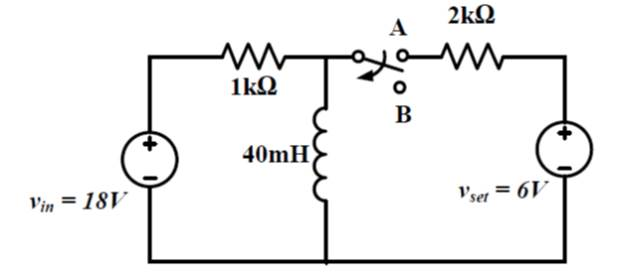
\includegraphics[width=0.5\textwidth]{Example2.jpg}
\caption{Circuit to accompany example 2}
\label{fig: Example2}
\end{figure}

(a) Find $i_L(0)$ --
(b) Redraw the circuit for $t>0$ and use KVL or KCL to derive the differential equation in terms of $i_L(t)$ --
(c) Use the integrating factor technique to find the general solution for $i_L(t)$--
(d) Use the initial condition (from part a) to find the particular solution for  $i_L(t)$

\soln{5in}{
\begin{figure} [h!]
\centering
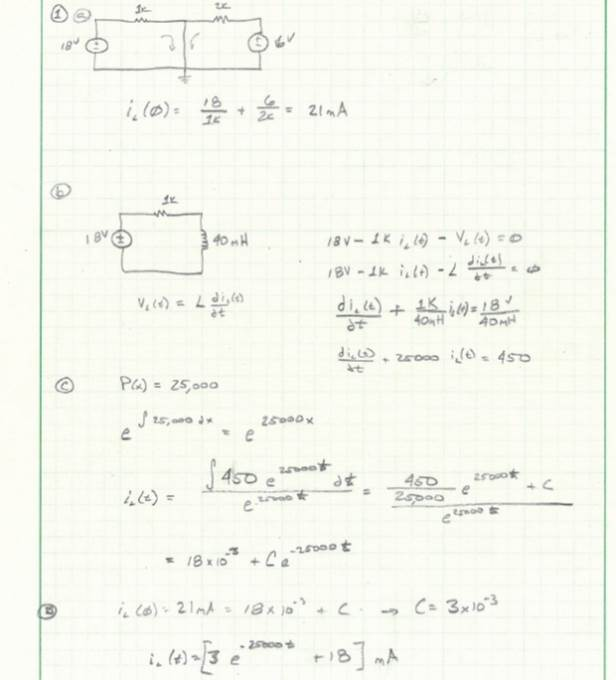
\includegraphics[width=0.8\textwidth]{Example2soln.jpg}
\end{figure}
}

\newpage
\clearpage
\pagebreak

\subsection{Example 3}
Answer the questions below for the circuit shown in Figure \ref{fig: Example3}
\begin{figure} [h!]
\centering
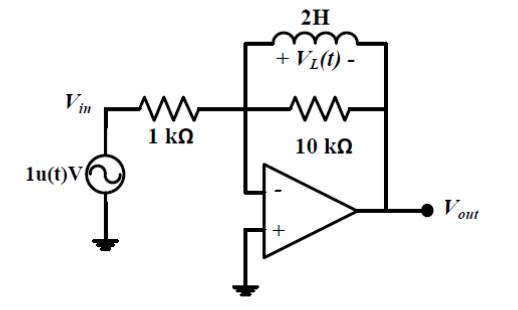
\includegraphics[width=0.5\textwidth]{Example3.jpg}
\caption{Circuit to accompany example 3}
\label{fig: Example3}
\end{figure}

(a) Find $i_L(0)$ (pay attention to the step function on the input)--
(b) Redraw the circuit for $t>0$ and use KVL or KCL to derive the differential equation in terms of $i_L(t)$ --
(c) Use the integrating factor technique to find the general solution for $i_L(t)$--
(d) Use the initial condition (from part a) to find the particular solution for  $i_L(t)$
(e) Write an equation for $v_{out}(t)$

\soln{5in}{
\begin{figure} [h!]
\centering
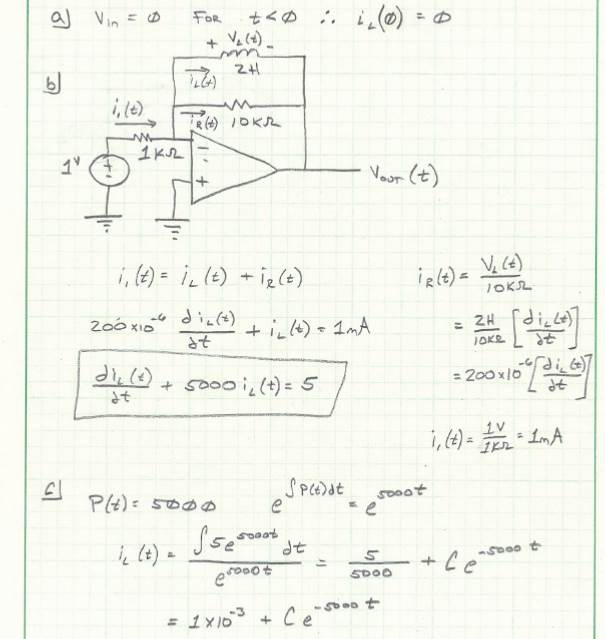
\includegraphics[width=0.7\textwidth]{Example3solnA.jpg}
\end{figure}
}

\newpage
\clearpage
\pagebreak

\soln{5in}{
\begin{figure} [h!]
\centering
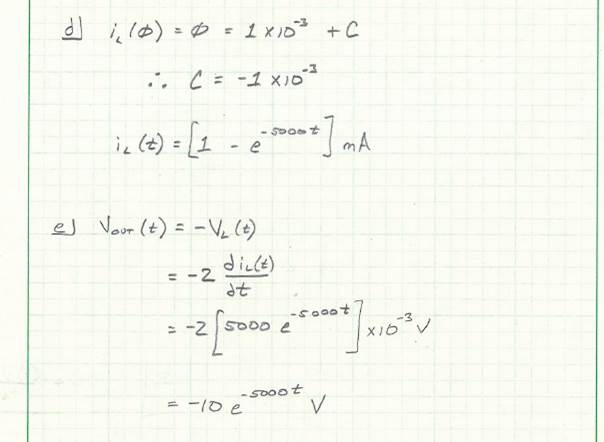
\includegraphics[width=1\textwidth]{Example3solnB.jpg}
\end{figure}
}


\newpage
\clearpage
\pagebreak

\subsection{Example 4}
For the circuit in Example 3 change the input to $\left[\cos(100t) + \cos(100,000t)\right]u(t)\ V$

(a) Use the integrating factor technique to find the general solution for $i_L(t)$--
(b) Use the initial condition (from part a) to find the particular solution for  $i_L(t)$--
(c) Write an equation for $v_{out}(t)$

Hint: You will need to use the following integral:
\[
\int e^{ax}\cos(bx) \partial x = \frac{e^{ax}}{a^2+b^2}\left[a\cos(bx) +b\sin(bx)  \right]
\]

\soln{5in}{
\begin{figure} [h!]
\centering
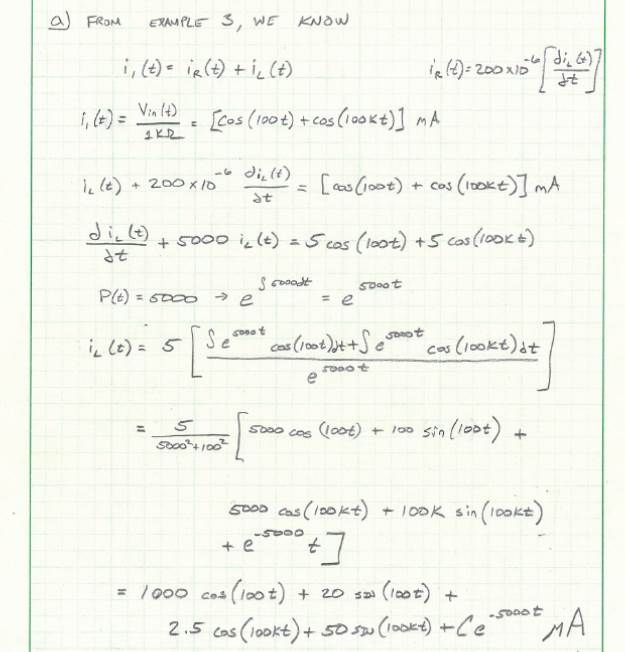
\includegraphics[width=1\textwidth]{Example4solnA.jpg}
\end{figure}
}

\newpage
\clearpage
\pagebreak

\soln{5in}{
\begin{figure} [h!]
\centering
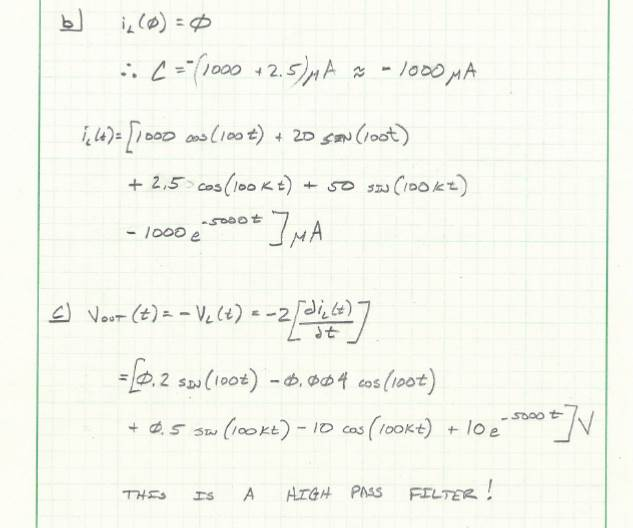
\includegraphics[width=1\textwidth]{Example4solnB.jpg}
\end{figure}
}

\newpage
\clearpage
\pagebreak



\end{document}


% Equation Array Example Code
%\begin
%{eqnarray}
%P_R &=& i_R^2R \nonumber \\
%P_R &=& (100\ mA)^2 \times 100\ \Omega \nonumber \\
%P_R &=& (100 \times 10^{-3}\ A)^2 \times 100\ \Omega \\
%P_R &=& 10000 \times 10^{-6}\ A^2  \times 100\ \Omega \nonumber \\
%P_R &=& 1\ W  \nonumber
%\end{eqnarray}

% Figure Example Code
%\begin{figure} [h!]
%\centering
%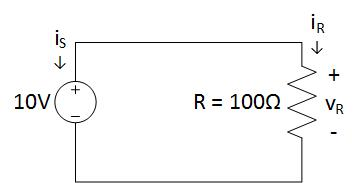
\includegraphics[width=0.5\textwidth]{OhmsLawExampleSolution.jpg}
%\caption{Ohm's Law example circuit}
%\label{fig: OhmsLawExampleSolution}
%\end{figure}

%Table Example Code
%\begin{table}[h]
%\centering
%\begin{tabular}{|l|c|c|}
%\hline
%Prefix & Abbreviation & Value \\
%\hline \hline
%Giga & $G$ & $10^9$ \\
%Mega & $M$ & $10^6$ \\
%Kilo & $k$ & $10^3$ \\
%\hline
%milli & $m$ & $10^{-3}$ \\
%micro & $\mu$ & $10^{-6}$ \\
%nano & $n$ & $10^{-9}$ \\
%pico & $p$ & $10^{-12}$ \\
%\hline
%\end{tabular}
%\caption{Engineering prefixes and values}
%\label{tab: Eng Prefixes}
%\end{table}
